%
% LaTeX report template 
%

\documentclass[a4paper,12pt]{article}
\renewcommand{\familydefault}{\rmdefault}
%\usepackage[T1]{fontenc}
\usepackage{graphicx}
\usepackage[english]{babel}
\usepackage[latin1]{inputenc}
\usepackage[margin=1in]{geometry}
\usepackage{fancyhdr}
\usepackage{mathptmx}
\usepackage{setspace}
\usepackage{enumitem}



\pagestyle{fancy}
\fancyhf{}

\fancyfoot[C]{\thepage}

\renewcommand{\headrulewidth}{0pt}
\renewcommand{\footrulewidth}{1pt}


%\setlength{\parindent}{4em}
%\setlength{\parskip}{1em}
\renewcommand{\baselinestretch}{1.55}
%
\begin{document}
%
\begin{center}
				
				
			
	{\LARGE Microservices Data Consistency Approaches: A tailored approach towards current limitations}
			
	\vspace{2cm}
			
	{\Large \bfseries Asim Riaz}
			
	\vspace{2cm}
				
	{\large 1732102}
				
	\vspace{3cm}
	
	{\Large  PhD CS}			
	\vspace{4cm}
	
	{\Large  Dr. Husnain Mansoor Ali}
	
	\vfill
		
	{\LARGE \bfseries SZABIST Karachi Campus	}
\end{center}






\thispagestyle{empty}

\newpage
\singlespacing % Reset line spacing to 1 from here on
\tableofcontents
\setstretch{1.55}   
 
\newpage
    
% This is a comment: in LaTeX everything that in a line comes
% after a "%" symbol is treated as comment
\section*{Abstract}
\addcontentsline{toc}{section}{\protect\numberline{}Abstract}%
% When adding * to \section, \subsection, etc... LaTeX will not assign
% a number to the section
Most organizations are shifting their monolithic architectures to microservices architecture. According to their domain model, the autonomous feature implements a data consistency model at the application level.  The software industry heavily relies on custom data consistency implementations using microservice architecture, even having multiple microservices data consistency frameworks and approaches available at their disposal. However, their adaption is limited. The study will explore the limits of existing data consistency approaches for microservices architecture. Find the gap which restricts the industry to adopt available solutions and propose a model to resolve the data consistency limitation



\paragraph{Keywords:}
Microservices Architecture, Monolithic Architecture, Data Consistency 
%\begin{verbatim}
%
%http://www.wisc.edu/writing/Handbook/ScienceReport.html
%
%\end{verbatim}


\section*{INTRODUCTION}
\addcontentsline{toc}{section}{\protect\numberline{}INTRODUCTION}%
The most crucial factor in the popularity of the microservices architectural style is its autonomous modularity.\cite{one, fifteen, cite-29} Any monolithic architecture can be easily transformed into microservices architecture by functional decomposition. This process attains strong isolation and provides scalability and variation of database systems, which helps deploy microservices in a broader spectrum. The fast-tracked adaptation of microservice style is the flexibility of designing service into any platform and vendor-neutral database system, which may help to increase its performance. The most important aspect of microservices architecture is usually deployed in a cloud environment. It allows new practices and cutting-edge technologies like lightweight containers. All services related to any domain can be easily maintained and deployed using container orchestration technologies (e.g., \cite{twentyfive}Docker Swarm, \cite{twentysix} Kubernetes, and \cite{twentyseven}Moses. It also encourages a \cite{twentyeight}DevOps environment which is industry top proven practices
Many small and medium-sized organizations are adopting microservices architecture because it is independent of the domain and size of the organization even system. It shows significant differences in benefits and adaptations of better practices and new technologies that implicitly cure legacy issues of monolithic architecture. \cite{sixteen} These new practices and technologies involve uncertainties, risks, and massive investment in process and infrastructure. To overcome the uncertainty and risk, the modularity of this architecture allows an organization's selective and gradual adaptation.
The gradual and selective transition allows an organization to incur more sophisticated solutions and infrastructure according to modern business demands. For example, an organization might consider adopting microservice architecture for fast delivery rather than flexible scalability because the system is running on a required and stable workload but unable to deliver fast delivery of new features. Therefore, an organization will focus more on the corresponding feature, and investment will be directed towards those advanced microservices infrastructure.\cite{cite-30} There is a significant difference between the supported advantages and practices available in the literature and the industry implementation and achieved benefits. It is necessary to discover the difference in industry adaptation for microservices architecture \cite{nine, eleven, five}


\section*{Microservice Architecture}
\begin{figure}[h!]
	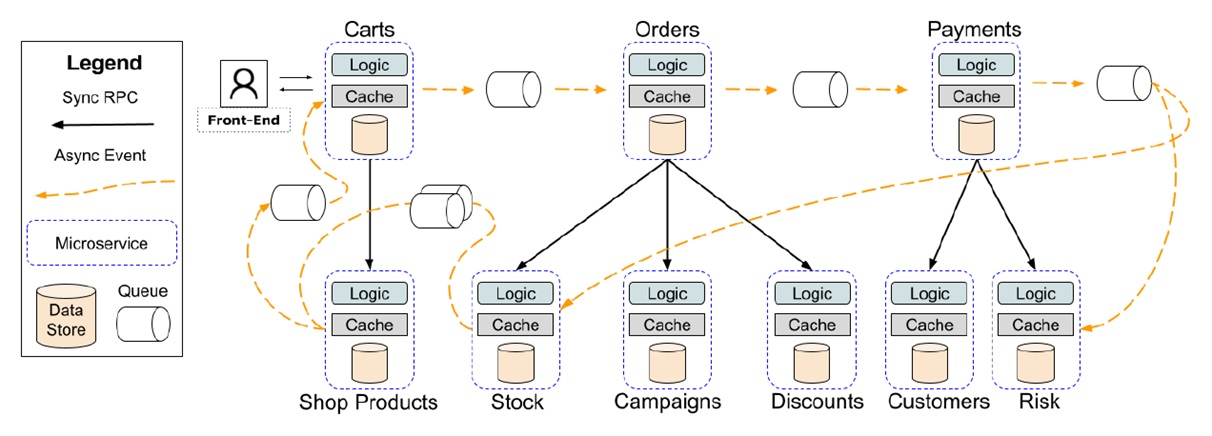
\includegraphics[width=\linewidth]{img/MicroserviceArchitecture.jpg}
	\caption{Microservices Architecture.\cite{one}}
	\label{fig:microarch}
\end{figure}
\addcontentsline{toc}{section}{\protect\numberline{}Microservice Architecture}%
The shift in architectural design of data-driven applications is due to the beginning of large-scale online services. It initiates the requirement of distributed applications with both software development and computational requirement concerning team organization.\cite{two} This situation promotes microservice architecture to take over traditional monolithic architecture because microservice architecture supports small-scale isolated services built and deployed independently. In contrast to this scenario, the conventional environment system is designed in a modular-based architecture, maintained centralized. We can analyze an e-commerce application to evaluate both architectures to depict the current scenario. In Figure 1, traditional architecture, a module is called which interns the next module or submodules to complete its functionality.\cite{cite-40, cite-35} e.g., a Cart module is responsible for to call Order module, which will call Stock, Campaign, and Discount modules sequentially. A transaction control protocol monitors all these modules. \cite{three, four}
 
In contrast to the direct function call, a microservices architecture communicates through remote calls such as asynchronous messages and HTTP-based protocol. \cite{cite-31} In case of new functionality or a bug fix, only redeployment of a microservice unit is required, whereas, in the case of monolithic architecture, a new build or patch involves the deployment of the whole application; in a similar context, microservices manages failures, each service is isolated in nature which limits the failure propagation to other services or building blocks. Moreover, every microservice handles its repository requirement in handling data concerning its format to fulfill the workload of the microservice. \cite{thirteen, fifteen} This adaptability is associated with the diligence of database architecture, and different services are maintained for the relational database management system and loosely structures NoSQL
For instance, microservices may use loosely structured databases like NoSQL for variable structure data management, whereas another microservice may utilize a relational model to implement constraints on the data incurred. This results in substantial modification of microservice architecture transaction processing systems compared to monolithic architecture. \cite{cite-32} Microservice architecture has an isolated environment that demands the decomposition of transactions into its service level. Otherwise, monolithic architecture transaction processing has well-defined steps for execution across modules.\cite{four, nine, ten}


\section*{PROBLEM BACKGROUND}
\addcontentsline{toc}{section}{\protect\numberline{}PROBLEM BACKGROUND}%

\section{Microservice Data Consistency}
 
Decentralized architecture helps microservices implement autonomy and isolation, but they have moved significantly away from traditional database management systems. \cite{three, four} This situation urges developers to implement data management logic at the application level. This open architecture of microservices allows developers to adjust all types of customizations required to handle any constraints. \cite{cite-33} The study focuses on exploring all those scenarios in which developers must implement those features dealt with by traditional mature database management systems.


\subsection{Data validation across microservices}
\begin{figure}[h!]
    \begin{center}
	    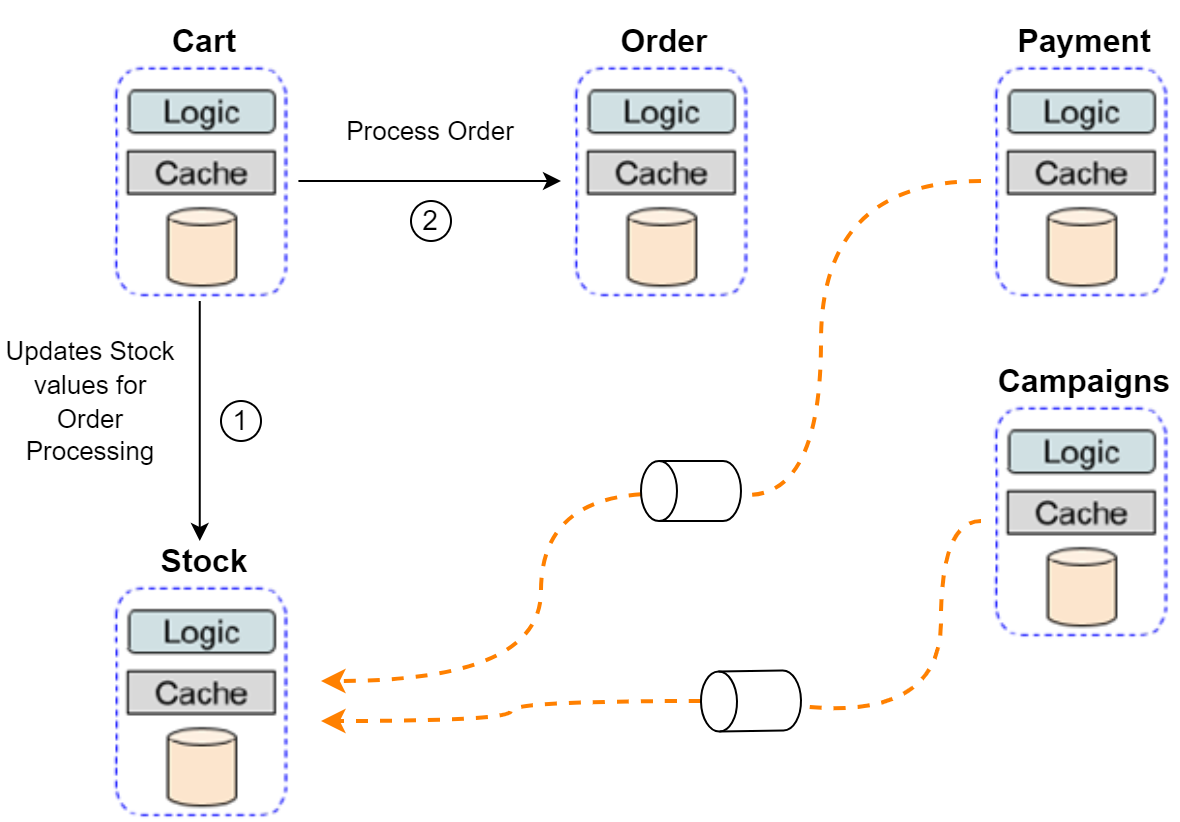
\includegraphics[width=0.7\columnwidth]{img/validation.png}
    \end{center}
	\caption{Data validation across microservices.}
	\label{fig:microarch}
\end{figure}
With the widespread data transactions in all microservices, the most crucial part is data validation across microservices. Take a scenario in Figure 2, in an Order Processing System. An order is processed in a cart for further processing. \cite{cite-34} It first validates the stock availability with a Sync RPC (synchronous Remote Procedure Call) and then processes the order for checkout. In the meantime, any other microservices executing simultaneously can update such stock service, which is already under process by another truncation. This scenario will create a concurrency anomaly that developers can handle at the application level in a microservices architecture. \cite{one, three, seven, twelve}


 

\subsection{Foreign Key Constraint }
\begin{figure}[h!]
    \begin{center}
	    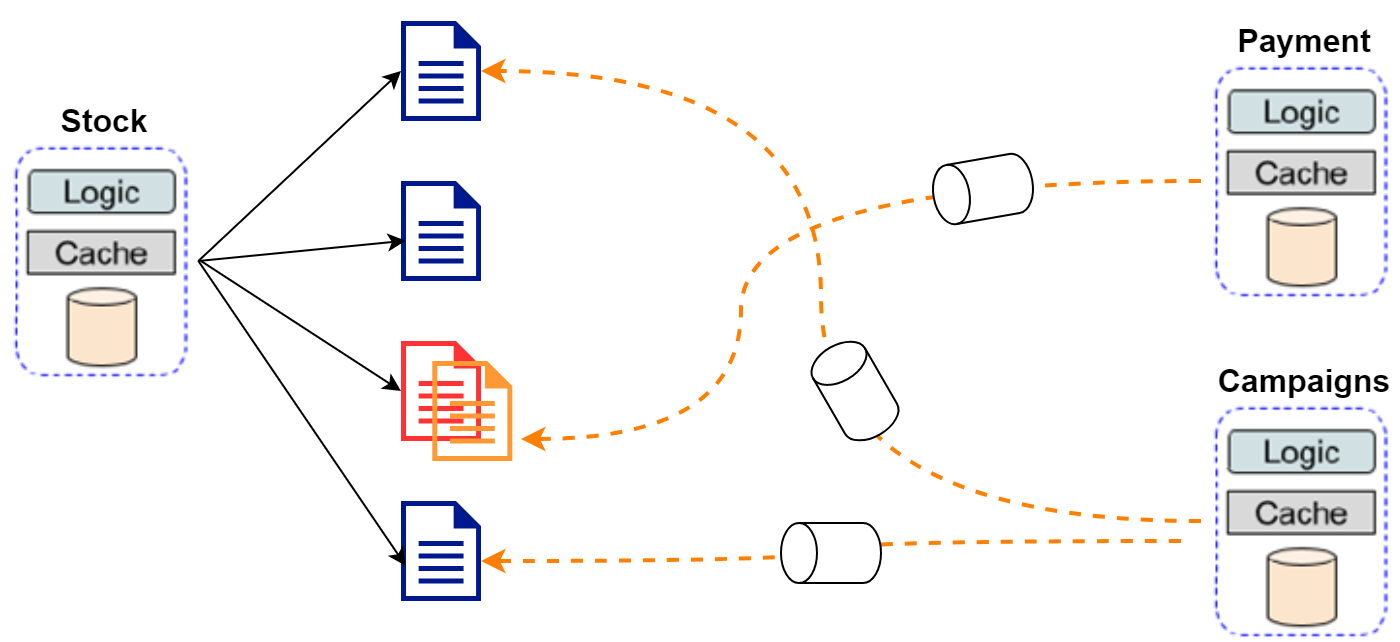
\includegraphics[width=0.7\columnwidth]{img/foreignkey.png}
    \end{center}
	\caption{Implicit Cross Microservice Associations.}
	\label{fig:microarch}
\end{figure}
The main approach which is directly dependent on microservices architecture is functional decomposition. The process of decomposition separates the database implementation of each service within its own boundaries. \cite{six, eight} This situation leads to implicit data association between multiple microservices or in a database management term foreign key constraint between multiple microservices. In Figure 3 stock microservice is accessed by multiple services asynchronously. For instance, stock service is accessed by multiple services asynchronously. \cite{cite-36, cite-38} If a service performs any such operation through which any of the master record is can cascade update or delete, that operation cannot be reflected to other transaction or services specifically in delete operation.\cite{seventeen}
To maintain data consistency developers, must enforce foreign key constraint at application level ensuring system consistency state explicitly. On the other hand, in most cases mostly this situation in microservices architecture is ignored or developers are not aware of the consequences. This type of constraints will cause high level of anomalies.\cite{one, three, four}

\subsection{Cross Microservices Data Retrieval}
\begin{figure}[h!]
    \begin{center}
	    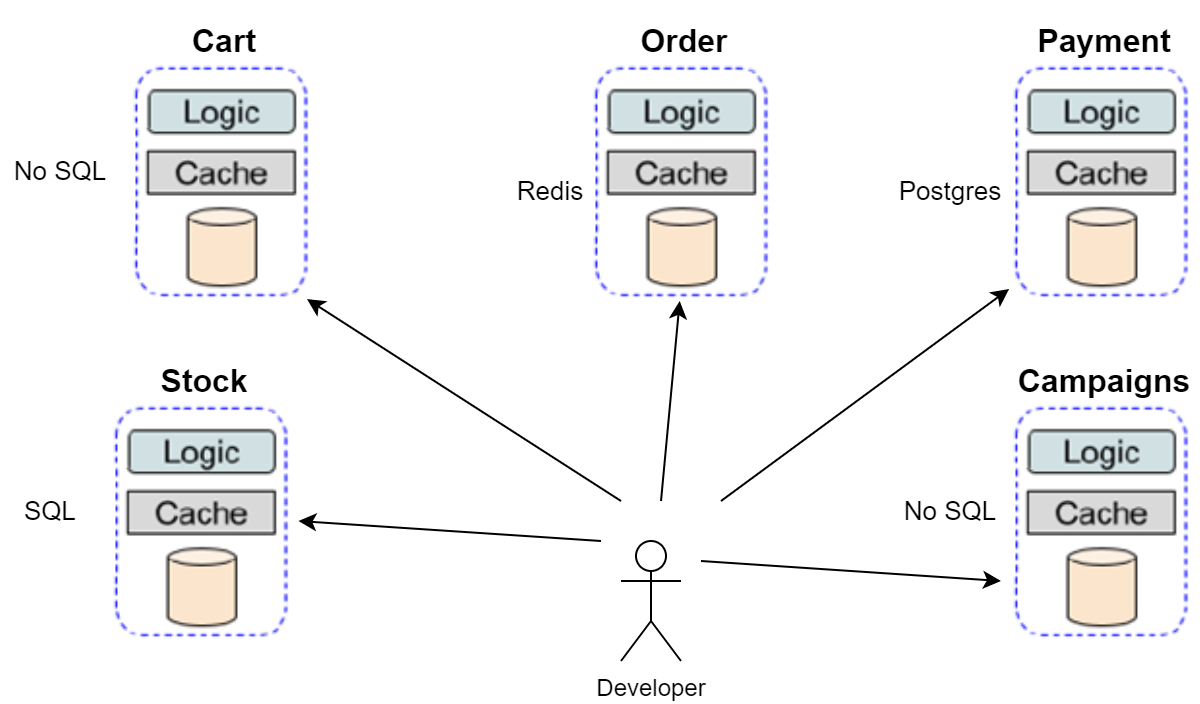
\includegraphics[width=0.7\columnwidth]{img/Queries.png}
    \end{center}
	\caption{Cross Microservice Queries.}
	\label{fig:microarch}
\end{figure}
The distributed nature of microservices architecture provides facilitation for online queries. Online queries were not popular in traditional monolithic systems because data is stored and maintained in a single source. The challenge of encapsulation data appears in distributed environment like microservices architecture. 
As shown in Figure 4, To resolve the challenge of data retrieval in microservices environment data aggregation techniques are employed spanning multiple microservices according to their underline databases. Another technique is used for data access in microservices environment is through middleware.\cite{cite-39} The middle-tier is employed in-between different microservices which is used to process functionality in application. The most critical aspect in these kinds of queries is the consistent state of the data. Maintaining consistency in data retrieval at application level is responsibility of developers in microservices environment. Besides, data consistency we don\' t have any specific methods of data retrieval on a particular state of different microservices which show the entire application view at a particular instance of time. Lastly, we don't have any method to ensure successful completion of all requests from multiple microservices. \cite{three, fourteen, eighteen}
 
\subsection{Feral Ordering}
\begin{figure}[h!]
    \begin{center}
	    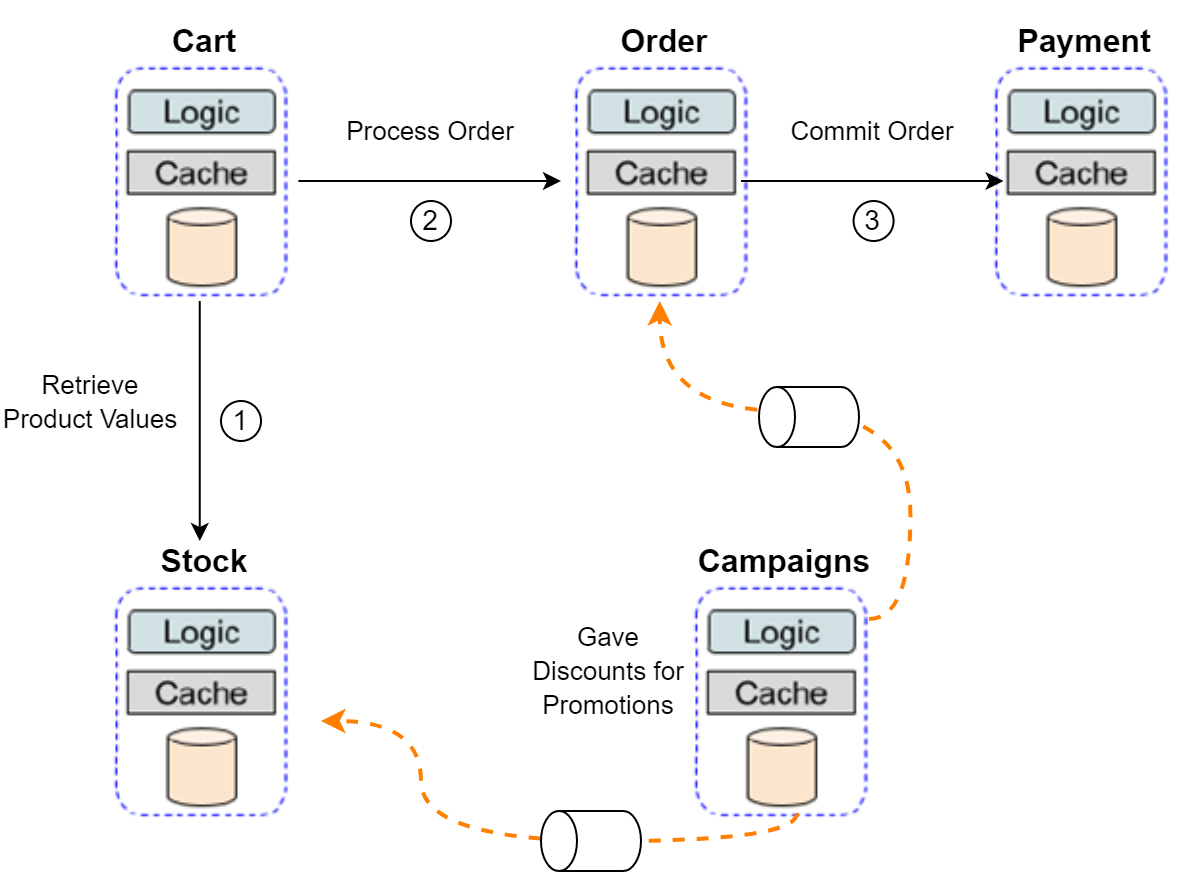
\includegraphics[width=0.7\columnwidth]{img/Feral.png}
    \end{center}
	\caption{Feral Ordering.}
	\label{fig:microarch}
\end{figure}
This consistency is related to the execution sequence of microservices. Let suppose an ecommerce application is working in a microservices architecture. Which multiple users can purchase different items in the system? For example, a user has multiple items selected in a cart to purchase. When a user is in process to check, meanwhile the price of one item was updated through any arbitrary microservice in that cart In Figure 5, Now in this situation two events can be handled. First, the price of the item should be update according to updated price. Second, price will be reflected on later order which will come after update of price.
In this scenario microservice architecture does not enforce any kind of constraint. This constraint is in the category of eventual consistency. Developers have to handle this type of constraint in application-level. Which will directly dependent application architecture of microservice workflow mechanism. \cite{one, three, twentyfour}

\section{Related Work}
\subsection{Saga Pattern}
The Saga pattern handle transaction in a distributed manner. Transaction control is dependent upon each microservices as compared to a whole transaction handling all microservices. This helps to reduce the dependency of transactions and support microservices architecture isolation environment. It does not ensure transactional guarantee like 2PC but take a long time to complete transaction requirement. In Saga local transactions works sequentially, where each transaction id controlled by a single microservice. Initialization stars from external event-based request. All transaction will be executed in a sequentially manner one after another. If any subsequent microservice failed to complete it transaction, a compensation actions will be triggered to roll back the transaction to maintain consistency. \cite{twentyone, twentytwo, twentythree}  

\subsection{Two-Phase Commit (2PC)}
This protocol is a technique to handle database transaction in a distributed environment like relational database management systems. It confirms the serialization of the transaction to maintain centralized atomic commit. It is well defined that this protocol performance degrades in high throughput systems like cloud computing or microservices. To maintain data constancy in microservice concurrency can be maintain in a decentralized manner like in every microservice individually. In 2PC, a coordinator transaction observes the whole business process integrity. If all sub transactions complete successfully, it commits the transaction successful. On other hand if any sub transaction fails to complete, the coordinator transaction calls rollback all successful transactions to a consistent state. The reason why 2PC is not efficient in cloud computing and microservices environment because it was difficult to maintain state for coordinator transaction to track sub transactions.     
In 2PC follows a rule in which all sub transaction should be available at the time of commit. If any sub transaction fails, the whole transaction cannot be completed. To ensure correctness of transaction 2PC sub transaction maintain locking mechanism which may lead to a critical situation and can affect the throughput of transaction. Another lacking in this technique that support for modern technologies is missing e.g., message broker and NoSQL databases \cite{twenty}

\subsection{SEATA}
SEATA is an open-source framework for handling distributed transactions based on java. SEATA works on different modes in which AT, XA, TCC, and Saga is included. It provides solutions based on domain model. It also implements a hybrid solution based on the requirement on certain condition. In SEATA XA mode is implemented as 2PC model and Saga works as it is. XA is the major feature of the framework which is totally unaware from the business code. It focuses on business transactions (SQL), so that it can generate rollback data after analyzing. In the first stage, all sub transaction or microservice involve in the transaction for local commit to generate rollback log. In second phase a global transaction works asynchronously to take decision for commit or rollback depending upon situation of all sub-transactions. In TCC works on Try, Confirm and Cancel basis. In try phase all sub-transaction participated in distributed transaction to acquire business resources. In confirm phase, if all sub-transaction were successful, it executes commit. Cancel phase initiate cancellation the business resource used in try phase \cite{nineteen}


 


\newpage
 
\section{Research Roadmap}
\begin{figure}[h!]
    \begin{center}
	    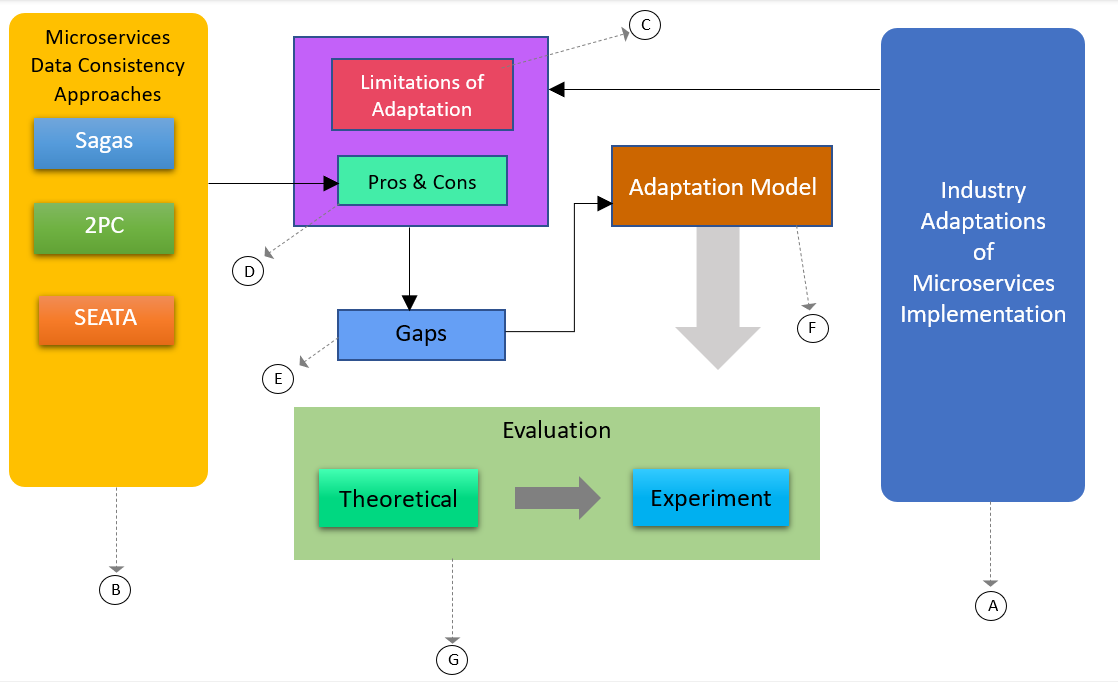
\includegraphics[width=\columnwidth]{img/roadmap.png}
    \end{center}
	\caption{Research Roadmap.}
	\label{fig:microarch}
\end{figure}

\begin{enumerate}[label=\Alph*.]
\item \textbf{Industry adaptation microservices Implementations:} This is the core of this study in which adaptations of microservices are evaluated:
\begin{itemize}
    \item Why are organizations adopting microservices very rapidly? 
    \item Factor involves in migration from monolithic to microservices architecture? 
    \item What data consistency issues were faced by practitioners / developers? 
\end{itemize}

\item \textbf{Microservice Data Consistency Approaches:} This area will explore all approaches available currently in industry for maintaining data consistency in a distributed environment.
\item \textbf{Limitation of adaptations:} What is the limitation of adopting microservices over monolithic architecture. Why almost every implementation is different from any other implementation in between organization
\item \textbf{Pros \& Corns:} It will explore pros \& corns of each Framework, Approach and practice used to maintain data consistency in microservices architecture
\item \textbf{Gaps:}The limitations of industry implementation and pros \& cons of frameworks, approaches and practices will identify the reasons why almost all implementations of microservices differ from each other. The most important part is why developers have different approaches in maintaining data consistency at application-level. Some organizations have fully or partially implemented these models, but they must customize to some extent.
\item \textbf{Adaptation Model:} This will be the contribution towards the problem of data consistency. It will focus the limitation of industry implementation. It also investigates those area due to which organization are not able to completely implement the present solution. The most important aspect of this model it would focuses open architecture of microservices architecture. A microservice do not need to be rewritten to adapt a particular model, rather than it would an improvisation to the current implementation.
\item \textbf{Evaluation:} This phase is used to test the desired adaptation model. There will be two stages to test this model. First stage will be a theoretical model which can define the steps of using or integrating this model. The next stage will be the simulation part in which a model will be experimented on its adaptation 
\end{enumerate}
 
\newpage

\section{Problem Statement}

Most organizations are shifting their monolithic architectures to microservices architecture. The autonomous feature tends to implement data consistency model at application level according to their domain model. Software industry heavily relies on custom data consistency implementations while using microservice architecture. Even having multiple microservices data consistency frameworks and approaches available at their disposal, however, their adaption is limited. The research will:
\begin{itemize}
     

\item	Pursue to identify the limitation of existing microservices data consistency approaches
\item	Segregate the limitations that hinder the adaptation of microservices data consistency approaches by industry
\item	Propose potential solutions to overcome selected limitations to increase industry adaptation of microservices data consistency approaches
\end{itemize}


\section{Hypothesis}
h\textsuperscript{1}: Microservices data consistency can be reduced by an adaptation model
\\
h\textsuperscript{0}: Microservices data consistency cannot be reduced by an adaptation model
\\

\section{Research Objective}
\begin{enumerate}
     
\item	Evaluate limitations of microservices data consistency approaches for industry adaptation
\item	Design and proposed adaptation model.
\item	Testing and evaluation of proposed adaptation model.
\end{enumerate}
\newpage
\section{Research Questions}
\begin{enumerate}
\item	What are the current limitations of microservices based data consistency approaches, and what adequacy are required to be addressed?
\item	How will proposed adaptation model cater towards the limitations of the current microservices practices?
\item	Which testing criteria and evaluation techniques be suitable to assess the proposed adaptation model?
\end{enumerate}

\section{Methodology}
\begin{figure}[h!]
    \begin{center}
	    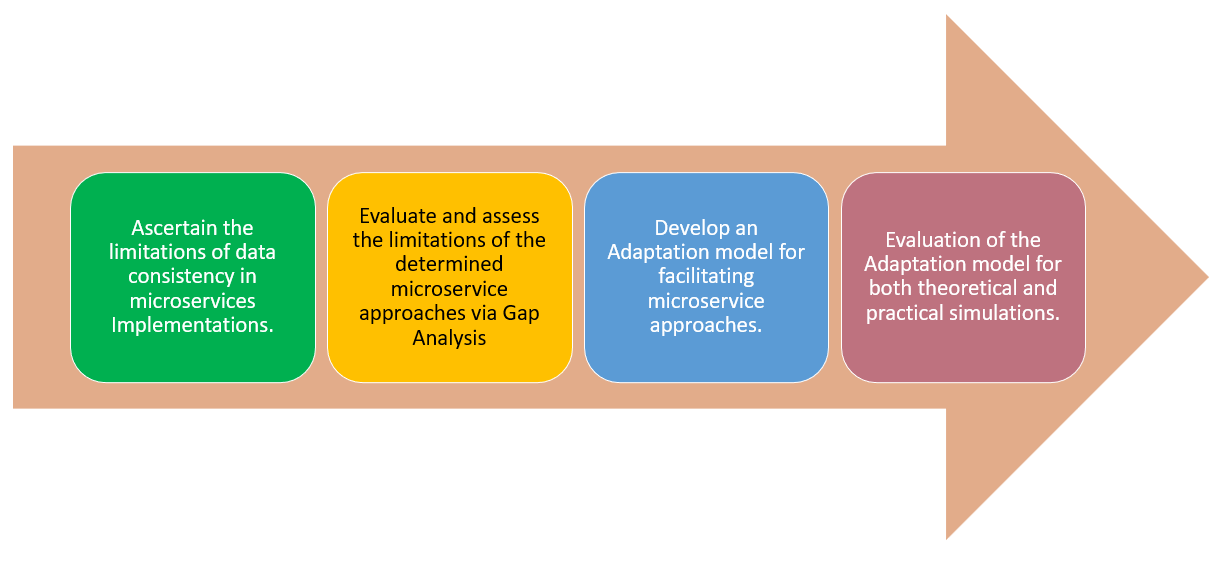
\includegraphics[width=\columnwidth]{img/methodology.png}
    \end{center}
	\caption{Methodology}
	\label{fig:microarch}
\end{figure}
\begin{enumerate}
\item	Ascertain the limitations of data consistency in microservices Implementations.
\item	Evaluate and assess the limitations of the determined microservice approaches via Gap Analysis
\item	Develop an Adaptation model for facilitating microservice approaches.
\item	Evaluation of the Adaptation model for both theoretical and practical simulations.
\end{enumerate}

 
 







\newpage


% TABLES

\setstretch{1.05}
\begin{thebibliography}{}
	
	\bibitem{one} Laigner, R., Zhou, Y., Salles, M.A.V., Liu, Y. and Kalinowski, M., 2021. Data Management in Microservices: State of the Practice, Challenges, and Research Directions. arXiv preprint arXiv:2103.00170.   
	
\bibitem{two}Xiang, Q., Peng, X., He, C., Wang, H., Xie, T., Liu, D., Zhang, G. and Cai, Y., 2021. No Free Lunch: Microservice Practices Reconsidered in Industry. arXiv preprint arXiv:2106.07321.

\bibitem{three}Waseem, M., Liang, P., Shahin, M., Ahmad, A. and Nassab, A.R., 2021. On the Nature of Issues in Five Open Source Microservices Systems: An Empirical Study. In Evaluation and Assessment in Software Engineering (pp. 201-210).

\bibitem{four}Baškarada, S., Nguyen, V. and Koronios, A., 2018. Architecting microservices: Practical opportunities and challenges. Journal of Computer Information Systems.

\bibitem{five}Laigner, R., Kalinowski, M., Diniz, P., Barros, L., Cassino, C., Lemos, M., Arruda, D., Lifschitz, S. and Zhou, Y., 2020, August. From a monolithic big data system to a microservices event-driven architecture. In 2020 46th Euromicro Conference on Software Engineering and Advanced Applications (SEAA) (pp. 213-220). IEEE.

\bibitem{six}Lesniak, A., Laigner, R. and Zhou, Y., 2021, June. Enforcing consistency in microservice architectures through event-based constraints. In Proceedings of the 15th ACM International Conference on Distributed and Event-based Systems (pp. 180-183).

\bibitem{seven}Akbulut, A. and Perros, H.G., 2019. Performance analysis of microservice design patterns. IEEE Internet Computing, 23(6), pp.19-27.

\bibitem{eight}Munonye, K. and Martinek, P., 2020, June. Evaluation of Data Storage Patterns in Microservices Archicture. In 2020 IEEE 15th International Conference of System of Systems Engineering (SoSE) (pp. 373-380). IEEE.

\bibitem{nine}Daja, D., 2020. Data Transformation: An Overview.

\bibitem{ten}Laigner, R., Zhou, Y. and Salles, M.A.V., 2021, June. A distributed database system for event-based microservices. In Proceedings of the 15th ACM International Conference on Distributed and Event-based Systems (pp. 25-30).

\bibitem{eleven}Bailis, P. and Ghodsi, A., 2013. Eventual consistency today: limitations, extensions, and beyond. Communications of the ACM, 56(5), pp.55-63.

\bibitem{twelve}Di Francesco, P., Lago, P. and Malavolta, I., 2018, April. Migrating towards microservice architectures: an industrial survey. In 2018 IEEE International Conference on Software Architecture (ICSA) (pp. 29-2909). IEEE.

\bibitem{thirteen}Taibi, D., Lenarduzzi, V. and Pahl, C., 2017. Processes, motivations, and issues for migrating to microservices architectures: An empirical investigation. IEEE Cloud Computing, 4(5), pp.22-32.

\bibitem{fourteen}Zhang, H., Li, S., Jia, Z., Zhong, C. and Zhang, C., 2019, March. Microservice architecture in reality: An industrial inquiry. In 2019 IEEE international conference on software architecture (ICSA) (pp. 51-60). IEEE.

\bibitem{fifteen}Haselböck, S., Weinreich, R. and Buchgeher, G., 2018, November. An expert interview study on areas of microservice design. In 2018 IEEE 11th Conference on Service-Oriented Computing and Applications (SOCA) (pp. 137-144). IEEE.

\bibitem{sixteen}Bogner, J., Fritzsch, J., Wagner, S. and Zimmermann, A., 2019, March. Microservices in industry: insights into technologies, characteristics, and software quality. In 2019 IEEE international conference on software architecture companion (ICSA-C) (pp. 187-195). IEEE.

\bibitem{seventeen}Ntentos, E., Zdun, U., Plakidas, K., Schall, D., Li, F. and Meixner, S., 2019, September. Supporting architectural decision making on data management in microservice architectures. In European Conference on Software Architecture (pp. 20-36). Springer, Cham.

\bibitem{eighteen}Shadija, D., Rezai, M. and Hill, R., 2017, September. Towards an understanding of microservices. In 2017 23rd International Conference on Automation and Computing (ICAC) (pp. 1-6). IEEE.

\bibitem{nineteen}seata.io. (n.d.). Seata. [online] Available at: https://seata.io/en-us/ [Accessed 2 Feb. 2022].

\bibitem{twenty}Fan, P., Liu, J., Yin, W., Wang, H., Chen, X. and Sun, H., 2020. 2PC*: a distributed transaction concurrency control protocol of multi-microservice based on cloud computing platform. Journal of Cloud Computing, 9(1), pp.1-22.

\bibitem{twentyone}Limon, X., Guerra-Hernández, A., Sánchez-García, A.J. and Arriaga, J.C.P., 2018, October. SagaMAS: a software framework for distributed transactions in the microservice architecture. In 2018 6th International Conference in Software Engineering Research and Innovation (CONISOFT) (pp. 50-58). IEEE.

\bibitem{twentytwo}D\"{u}rr, K., Lichtenth\"{a}ler, R. and Wirtz, G., 2021. An Evaluation of Saga Pattern Implementation Technologies. In ZEUS (pp. 74-82).

\bibitem{twentythree}Malyuga, K., Perl, O., Slapoguzov, A. and Perl, I., 2020, April. Fault tolerant central saga orchestrator in RESTful architecture. In 2020 26th Conference of Open Innovations Association (FRUCT) (pp. 278-283). IEEE.

\bibitem{twentyfour}Bailis, P., Fekete, A., Franklin, M.J., Ghodsi, A., Hellerstein, J.M. and Stoica, I., 2015, May. Feral concurrency control: An empirical investigation of modern application integrity. In Proceedings of the 2015 ACM SIGMOD International Conference on Management of Data (pp. 1327-1342).

\bibitem{twentyfive}Docker (2018). Enterprise Application Container Platform | Docker. [online] Docker. Available at: https://www.docker.com/.

\bibitem{twentysix}Kubernetes (2019). Production-Grade Container Orchestration. [online] Kubernetes.io. Available at: https://kubernetes.io/.

\bibitem{twentyseven}Apache Mesos. (n.d.). Apache Mesos. [online] Available at: https://mesos.apache.org/.

\bibitem{twentyeight}DevOps.com. (n.d.). Home. [online] Available at: https://devops.com/ [Accessed 2 Feb. 2022].

\bibitem{cite-29}Di Francesco, P., Malavolta, I. and Lago, P., 2017, April. Research on architecting microservices: Trends, focus, and potential for industrial adoption. In 2017 IEEE International Conference on Software Architecture (ICSA) (pp. 21-30). IEEE.

\bibitem{cite-30}Esposito, C., Castiglione, A. and Choo, K.K.R., 2016. Challenges in delivering software in the cloud as microservices. IEEE Cloud Computing, 3(5), pp.10-14.
	
\bibitem{cite-31}Yarygina, T. and Bagge, A.H., 2018, March. Overcoming security challenges in microservice architectures. In 2018 IEEE Symposium on Service-Oriented System Engineering (SOSE) (pp. 11-20). IEEE.
	
\bibitem{cite-32}Taibi, D. and Lenarduzzi, V., 2018. On the definition of microservice bad smells. IEEE software, 35(3), pp.56-62.
	
\bibitem{cite-33}Richards, M., 2016. Microservices antipatterns and pitfalls. O'Reilly Media, Incorporated.
	
\bibitem{cite-34}Soldani, J., Tamburri, D.A. and Van Den Heuvel, W.J., 2018. The pains and gains of microservices: A systematic grey literature review. Journal of Systems and Software, 146, pp.215-232.
	
\bibitem{cite-35}Rademacher, F., Sorgalla, J. and Sachweh, S., 2018. Challenges of domain-driven microservice design: a model-driven perspective. IEEE Software, 35(3), pp.36-43.
	
\bibitem{cite-36}Hassan, S. and Bahsoon, R., 2016, June. Microservices and their design trade-offs: A self-adaptive roadmap. In 2016 IEEE International Conference on Services Computing (SCC) (pp. 813-818). IEEE.
	
\bibitem{cite-37}Bogner, J., Fritzsch, J., Wagner, S. and Zimmermann, A., 2019, March. Microservices in industry: insights into technologies, characteristics, and software quality. In 2019 IEEE international conference on software architecture companion (ICSA-C) (pp. 187-195). IEEE.
	
\bibitem{cite-38}Ford, N., 2018. The State of Microservices Maturity-Survey Results.
	
\bibitem{cite-39}Kleppmann, M., Beresford, A.R. and Svingen, B., 2019. Online event processing: Achieving consistency where distributed transactions have failed. Queue, 17(1), pp.116-136.
	
\bibitem{cite-40}Helland, P., 2020. Data on the Outside vs. Data on the Inside: Data kept outside SQL has different characteristics from data kept inside. Queue, 18(3), pp.43-60.

\end{thebibliography}

\end{document}
